
\section{Position \textit{vs.}~Time Graphs\footnote{
1990-93 Dept. of Physics and Astronomy, Dickinson College. Supported by FIPSE
(U.S. Dept. of Ed.) and NSF. Portions of this material may have been modified
locally and may not have been classroom tested at Dickinson College.
}}

\makelabheader %(Space for student name, etc., defined in master.tex or labmanual_formatting_commands.tex)

\bigskip

\textbf{Objectives} 

\begin{itemize}[nosep]
\item To learn about two of the ways that physicists can describe motion in one dimension-words
and graphs. 
\item To learn how to relate graphs of position \textit{vs.}~time to the motions they represent.
\end{itemize}

\bigskip

\textbf{Apparatus} 

\begin{itemize}[nosep]
\item Pasco 550 Interface
\item Ultrasonic motion detector 
\item \textit{Capstone} software (\filename{P\_Graphs.cap} experiment file)
\item Wooden board
\item Masking tape for marking distances
\end{itemize}

\bigskip

\textbf{Introduction} 

The focus of this unit on kinematics is to be able to describe your position
as a function of time using words and graphs. You will use a motion detector
attached to a computer in the laboratory to learn to describe one-dimensional
motion.

The ultrasonic motion detector sends out a series of sound pulses that are of
too high a frequency to hear. These pulses reflect from objects in the vicinity
of the motion detector and some of the sound energy returns to the detector.
The computer is able to record the time it takes for reflected sound waves to
return to the detector and then, by knowing the speed of sound in air, figure
out how far away the reflecting object is. There are several things to watch
out for when using a motion detector. (1) Do not get closer than 0.15 meters
from the detector because it cannot record reflected pulses which come back
too soon. (2) The ultrasonic waves come out in a cone of about 15\( ^{\circ } \).
It will see the closest object. Be sure there is a clear path between the object
whose motion you want to track and the motion detector. (3) The motion detector
is very sensitive and will detect slight motions. You can try to glide smoothly
along the floor, but don't be surprised to see small bumps in velocity graphs.
(4) Some objects like bulky sweaters are good sound absorbers and may not be
``seen'' well by a motion detector. Hold a wooden board in front of you when 
doing the activities below so the motion detector can see a smooth surface.

\textbf{Position \textit{vs.}~Time Graphs of Your Motion }

The purpose of this unit is to learn how to relate graphs of position as a function
of time to the motions they represent. How does a position \textit{vs.}~time graph look
when you move slowly? Quickly? What happens when you move toward the motion
detector? Away? After completing the next few activities, you should be able
to look at a position \textit{vs.}~time graph and describe the motion of the object.
You should also be able to look at the motion of an object and sketch a graph
representing that motion.

Note that the motion detector measures the distance of an object from the detector,
and that the motion detector is located at the origin of each graph. It is common
to refer to the distance of an object from some origin as the position of the
object. Therefore, it is better to refer to these graphs as position \textit{vs.}~time
graphs than distance \textit{vs.}~time graphs.

You will use the \textit{Capstone} software to do the following activities.
Launch the \filename{P\_Graphs.cap} file by going to the \filename{\coursefolder} folder on the desktop. 
To start a data run, click the \textbf{Record} button. To stop a data run,
click the \textbf{Stop} button. After a data run, the graph can be expanded
by clicking on the \textbf{Scale to fit} button in the upper left corner of
the Graph window. Multiple data sets can be displayed on the same graph. Data
can be removed from the graph by opening the \textbf{Delete Last Run} menu on the \textbf{Controls} palette 
 (at bottom of screen) and selecting \textit{delete all runs} or \textit{delete run number x}.
  When you are finished with the activities, choose \textbf{Exit} from the \textbf{File} menu
and do not save this activity.

Before you begin the activities, you should mark a position scale on the floor.
To do this, position one person at approximately 1 meter in front of the motion
detector and take data for 1 second. The computer will display a horizontal
line showing the position measured by the detector. The person standing in front
of the detector should then adjust his/her position and the procedure repeated
until the 1 meter position is established. Mark the 1 meter position on the
floor with a piece of masking tape and then mark the 2, 3 and 4 meter positions
using the 2 meter stick.

\textbf{Activity 1: Making Position \textit{vs.}~Time Graphs }

Make position-time graphs for the following motions and sketch the graph you
observe in each case:

(a) Starting at 0.5 m, walk away from the origin (i.e., the detector) slowly
and steadily.

%\vspace{0.3cm}
%{\par\centering 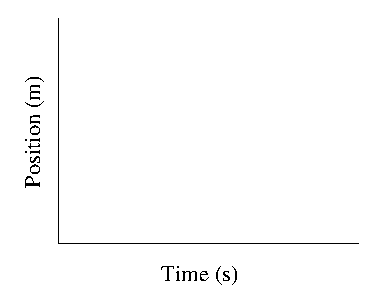
\includegraphics{position/position_fig1.eps} \par}
%\vspace{0.3cm}
\begin{lab_axis}*[lab_noticks_1quad,
	height = {2.0in}, width = {2.5in},
	xlabel={Time},
	ylabel={Position},
	]
\end{lab_axis}

(b) Walk away from the origin medium-fast and steadily.

%\vspace{0.3cm}
%{\par\centering 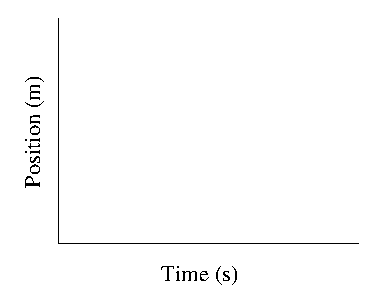
\includegraphics{position/position_fig1.eps} \par}
%\vspace{0.3cm}
\begin{lab_axis}*[lab_noticks_1quad,
	height = {2.0in}, width = {2.5in},
	xlabel={Time},
	ylabel={Position},
	]
\end{lab_axis}

(c) Walk toward the detector (origin) slowly and steadily.

%\vspace{0.3cm}
%{\par\centering 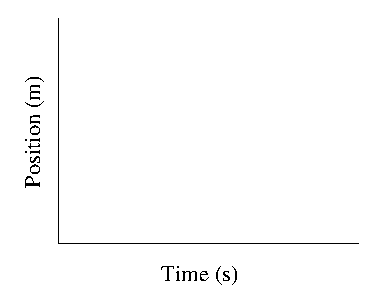
\includegraphics{position/position_fig1.eps} \par}
%\vspace{0.3cm}
\begin{lab_axis}*[lab_noticks_1quad,
	height = {2.0in}, width = {2.5in},
	xlabel={Time},
	ylabel={Position},
	]
\end{lab_axis}

(d) Describe the difference between the graph you made by walking away slowly
and the one made by walking away more quickly.
\answerspace{20mm}

(e) Describe the difference between the graph made by walking toward and the
one made walking away from the motion detector.
\answerspace{20mm}

\textbf{Activity 2: Predicting a Position \textit{vs.}~Time Graph} 

(a) Suppose your were to start 1.0 m in front of the detector and walk away
slowly and steadily for 4 seconds, stop for 4 seconds, and then walk toward
the detector quickly. Sketch your prediction on the axes below using a dashed
line.

%\vspace{0.3cm}
%{\par\centering 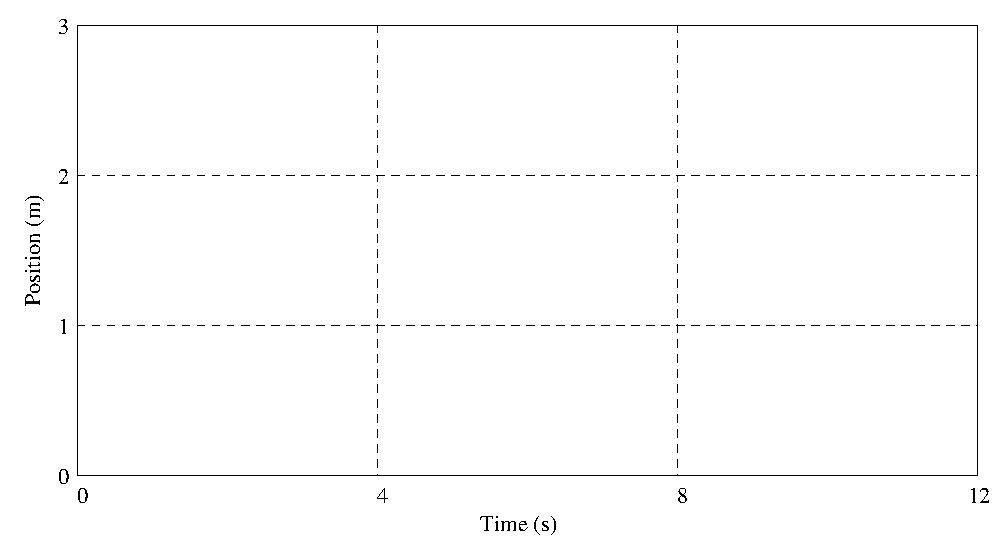
\includegraphics{position/position_fig2.eps} \par}
%\vspace{0.3cm}
\begin{lab_axis}*[lab_grid,
	height = {3in},
	width = {6in},
	xlabel={Time (s)},
	ylabel={Position (m)},
	xmin=0, xmax=12,
	ymin=0, ymax=3,
	xtick distance = 4,
%	ytick distance = 1,
	minor y tick num=1,
	minor x tick num=3,
	]
\end{lab_axis}

(b) Test your prediction by moving in the way described and making a graph of
your motion with the motion detector. Sketch the trace of your actual motion
on the above graph with a solid line. 

(c) Is your prediction the same as the final result? If not, describe how you
would move to make a graph that looks like your prediction.
\answerspace{20mm}

\pagebreak[2]
\textbf{Activity 3: Matching Position \textit{vs.}~Time Graphs}

%\vspace{0.3cm}
%{\par\centering 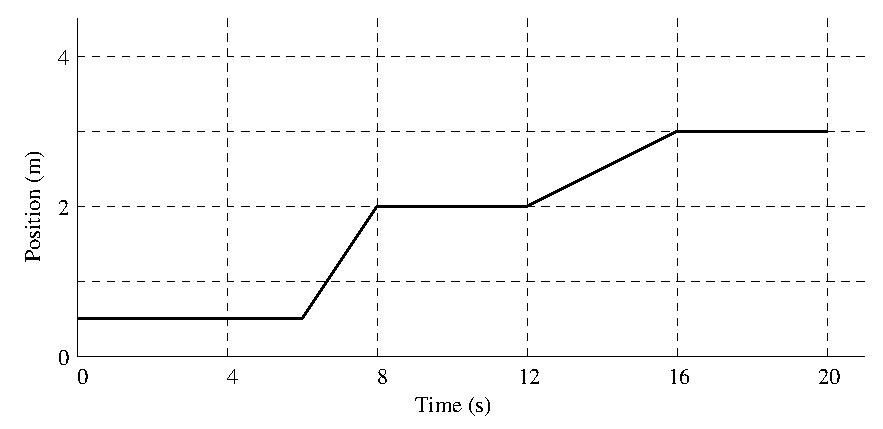
\includegraphics[width=0.7\textwidth]{position/position_fig3.eps} \par}
%\vspace{-0.1cm}
\begin{lab_axis}*[lab_grid,
	height = {2.5in},
	width = {5in},
	xlabel={Time (s)},
	ylabel={Position (m)},
	xmin=0, xmax=20,
	ymin=0, ymax=4,
	xtick distance = 4,
	ytick distance = 2,
	minor y tick num=1,
	minor x tick num=1,
	]
\addplot coordinates{(0,0.5) (6,0.5) (8,2) (12,2) (16,3) (20,3)};
\end{lab_axis}

(a) Describe in your own words how you would move in order to match the graph
shown above.
\answerspace{15mm}

(b) Move to match the above graph on the computer screen. You may try a number
of times. It helps to work as a team. Get the times right. Get the positions
right. Do this for yourself. (Each person in your group should do his or her
own match.) You will not learn very much by just watching!

(c) What was the difference in the way you moved to produce the two differently
sloped parts of the graph you just matched?
\answerspace{15mm}

(d) Make curved position \textit{vs.}~time graphs like those shown below.

%\vspace{0.3cm}
%{\par\centering 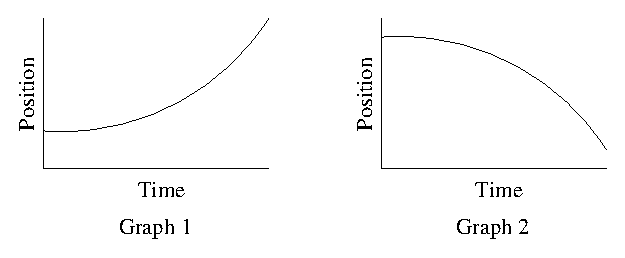
\includegraphics[width=0.5\textwidth]{position/position_fig4.eps} \par}
%\vspace{-0.1cm}
\begin{center}
\begin{lab_axis}[lab_noticks_1quad,
	height = {1.5in}, width = {2in},
	xlabel={Time},
	ylabel={Position},
	title={Graph 1},
	]
\addplot[domain=0:0.9] {0.8*x^2 + 0.2};
\end{lab_axis}
\hspace{0.5in}
\begin{lab_axis}[lab_noticks_1quad,
	height = {1.5in}, width = {2in},
	xlabel={Time},
	ylabel={Position},
	title={Graph 2},
	]
\addplot[domain=0:0.9] {-0.8*x^2 + 0.9};
\end{lab_axis}
\end{center}
%\vspace{-2em}

%\newpage
(e) Describe how you must move to produce a position \textit{vs.}~time graph with each
of the shapes shown.

Graph 1 answer:
\answerspace{10mm}

Graph 2 answer:
\answerspace{10mm}

\pagebreak[2]
(f) What is the general difference between motions which result in a straight-line
position \textit{vs.}~time graph and those that result in a curved-line position vs.
time graph?
\answerspace{15mm}

\pagebreak[2]
\textbf{Homework} 

Answer the following questions in the spaces provided.

1.What do you do to create a horizontal line on a position-time graph?

%\vspace{0.3cm}
%{\par\raggedright 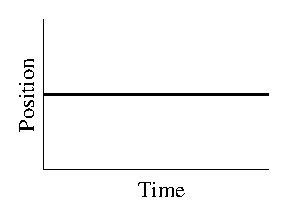
\includegraphics{position/position_fig5.eps} \par}
%\vspace{0.3cm}
\begin{lab_axis}[lab_noticks_1quad,
	height = {1.6in}, width = {2.0in},
	xlabel={Time},
	ylabel={Position},
	]
\addplot[domain=0:0.9] {0.5};
\end{lab_axis}

2. How do you walk to create a straight line that slopes up?

%\vspace{0.3cm}
%{\par\raggedright 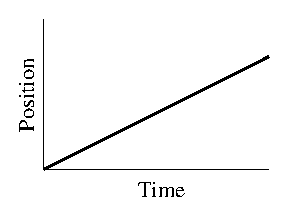
\includegraphics{position/position_fig6.eps} \par}
%\vspace{0.3cm}
\begin{lab_axis}[lab_noticks_1quad,
	height = {1.6in}, width = {2.0in},
	xlabel={Time},
	ylabel={Position},
	]
\addplot[domain=0:0.9] {x};
\end{lab_axis}

3. How do you walk to create a straight line that slopes down?

%\vspace{0.3cm}
%{\par\raggedright 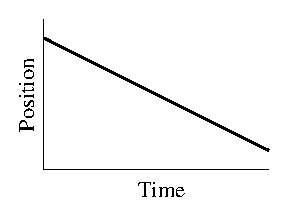
\includegraphics{position/position_fig7.eps} \par}
%\vspace{0.3cm}
\begin{lab_axis}[lab_noticks_1quad,
	height = {1.6in}, width = {2.0in},
	xlabel={Time},
	ylabel={Position},
	]
\addplot[domain=0:0.9] {0.9 - 0.8*x};
\end{lab_axis}

4. How do you move so the graph goes up steeply at first, then continues up
gradually?

%\vspace{0.3cm}
%{\par\raggedright 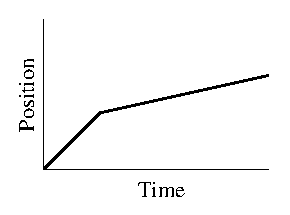
\includegraphics{position/position_fig8.eps} \par}
%\vspace{0.3cm}
\begin{lab_axis}[lab_noticks_1quad,
	height = {1.6in}, width = {2.0in},
	xlabel={Time},
	ylabel={Position},
	]
\addplot coordinates{(0,0) (0.25, 0.4) (0.9,0.7)};
\end{lab_axis}

5. How do you walk to create a U-shaped graph?

%\vspace{0.3cm}
%{\par\raggedright 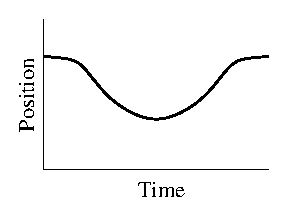
\includegraphics{position/position_fig9.eps} \par}
%\vspace{0.3cm}
\begin{lab_axis}[lab_noticks_1quad,
	height = {1.6in}, width = {2.0in},
	xlabel={Time},
	ylabel={Position},
	]
\addplot [smooth, tension=0.95] coordinates{(0,0.8) (0.2, 0.7) (0.5,0.25) (0.8, 0.7) (1.0, 0.8)};
\end{lab_axis}

\pagebreak[2]
Answer the following about the two objects A and B, whose motion produced
the following position-time graphs.

6. (a) Which object is moving faster? (b) Which starts ahead? Define what you
mean by ``ahead.''

(c) What does the intersection mean?

%\vspace{0.3cm}
%{\par\raggedright 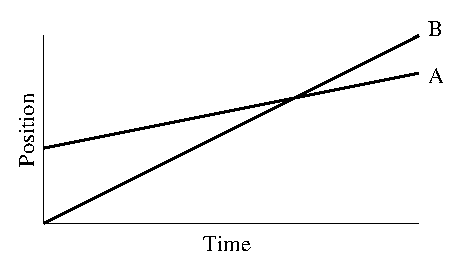
\includegraphics{position/position_fig10.eps} \par}
%\vspace{0.3cm}
\begin{lab_axis}[lab_noticks_1quad,
	height = {1.9in}, width = {2.8in},
	xlabel={Time},
	ylabel={Position},
	]
\addplot coordinates {(0,0.0) (0.9,0.9)} node[right] {B};
\addplot coordinates {(0,0.4) (0.9,0.7)} node[right] {A};
\end{lab_axis}

7. (a) Which object is moving faster? (b) Which object has a negative velocity
according to the convention we have established?

%\vspace{0.3cm}
%{\par\raggedright 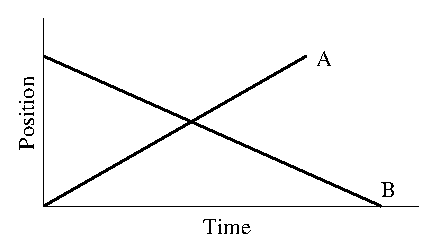
\includegraphics{position/position_fig11.eps} \par}
%\vspace{0.3cm}
\begin{lab_axis}[lab_noticks_1quad,
	height = {1.9in}, width = {2.8in},
	xlabel={Time},
	ylabel={Position},
	]
\addplot coordinates {(0,0.0) (0.9,0.9)} node[right] {A};
\addplot coordinates {(0,0.6) (0.9,0.3)} node[right] {B};
\end{lab_axis}

8. (a) Which object is moving faster? (b) Which starts ahead? Define what you
mean by ``ahead.''

%\vspace{0.3cm}
%{\par\raggedright 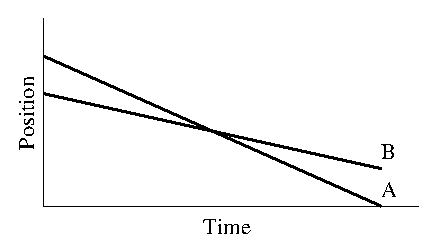
\includegraphics{position/position_fig12.eps} \par}
%\vspace{0.3cm}
\begin{lab_axis}[lab_noticks_1quad,
	height = {1.9in}, width = {2.8in},
	xlabel={Time},
	ylabel={Position},
	]
\addplot coordinates {(0,0.9) (0.9,0.1)} node[right] {A};
\addplot coordinates {(0,0.6) (0.9,0.3)} node[right] {B};
\end{lab_axis}

Sketch the position-time graph corresponding to each of the following descriptions
of the motion of an object.

9. The object moves with a steady (constant) velocity away from the origin.

%\vspace{0.3cm}
%{\par\centering 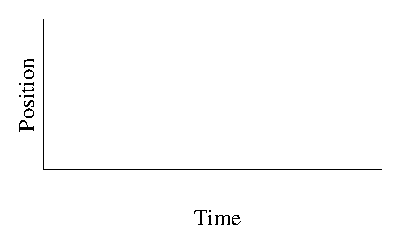
\includegraphics{position/position_fig13.eps} \par}
%\vspace{0.3cm}
\begin{lab_axis}*[lab_noticks_1quad,
	height = {1.8in}, width = {2.8in},
	xlabel={Time},
	ylabel={Position},
	]
\end{lab_axis}

\pagebreak
10. The object is standing still.

\begin{lab_axis}*[lab_noticks_1quad,
	height = {1.8in}, width = {2.8in},
	xlabel={Time},
	ylabel={Position},
	]
\end{lab_axis}

11. The object moves with a steady (constant) velocity toward the origin for
5 seconds and stands still for 5 seconds.

\begin{lab_axis}*[lab_noticks_1quad,
	height = {1.8in}, width = {2.8in},
	xlabel={Time},
	ylabel={Position},
	]
\end{lab_axis}

12. The object moves with a steady velocity away from the origin for 5 seconds,
then reverses direction and moves at the same speed toward the origin for 5
seconds.

\begin{lab_axis}*[lab_noticks_1quad,
	height = {1.8in}, width = {2.8in},
	xlabel={Time},
	ylabel={Position},
	]
\end{lab_axis}

13. The object moves away from the origin, starting slowly and speeding up.

\begin{lab_axis}*[lab_noticks_1quad,
	height = {1.8in}, width = {2.8in},
	xlabel={Time},
	ylabel={Position},
	]
\end{lab_axis}


